\section{Artificial Neural Network (ANN)}
Yapay sinir ağları, biyolojik sinir ağlarından esinlenerek oluşturulan matematiksel algoritmaları ifade eder. Bu algoritmalar, insan beyninin nöronlarının karmaşık bir şekilde birbirleriyle etkileşim içinde çalışmasını taklit eder. Girdi verilerini işleyerek öğrenme süreciyle desenleri tanımlar ve sonuçları tahmin etmek için kullanılır.

Yapay sinir ağları, birbirine bağlı bir dizi katman içeren bir yapıya sahiptir. Her bir katman, yapay sinir hücreleri veya nöronlar tarafından temsil edilir. Her bir nöron, girdi verilerini alır, ağırlıklarla çarpılır, bir aktivasyon fonksiyonuna uygulanır ve çıktıyı üretir. Bu işlem, ağın her katmanında tekrarlanır ve sonuç olarak bir çıktı üretilir.

\begin{figure}[ht]
    \centering
    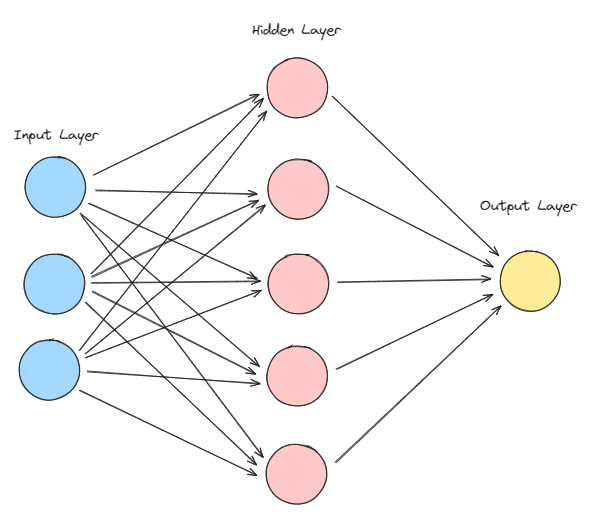
\includegraphics[width=0.7\textwidth]{images/ann_architecture.png}
    \caption{ANN mimarisi.}
    \label{fig:enter-label}
\end{figure}

Bir sinir ağı içerisindeki şunlar bulunur:

\begin{itemize}
	\item \textbf{Katmanlar:} Sinir ağları katmanlar halinde organize edilir. Girdi katmanı, gizli katman ve çıktı katmanı olmak üzere üç katman türü bulunur.
	\item \textbf{Nöronlar:} Nöronlar bir sinir ağındaki temel işlem birimleridir. Girdileri alırlar, ağırlıkları uygularlar ve bir aktivasyon fonksiyonuna göre aktive olarak bir çıktı üretirler.
	\item \textbf{Ağırlıklar:} Bağlı nöronlar arasındaki etkinin gücünü ve yönünü belirlerler ve eğitim sırasında ayarlanırlar.
	\item \textbf{Bias:} Bias, tüm girdiler sıfır olduğunda bile nöronların etkinleşmesine izin vererek onlara esneklik sağlar. Bir katmandaki her nöronun tipik olarak ilişkili bir bias terimi vardır.
	\item \textbf{Aktivasyon Fonksiyonları:} Aktivasyon fonksiyonları nöronların çıkışına doğrusal olmayan bir özellik katar.
\end{itemize}

Bir ANN tipik olarak 3 katmandan oluşur:

\begin{itemize}
    \item \textbf{Input Layer (Girdi Katmanı):} Girişin ağa beslendiği yerdir. Giriş katmanındaki nöronların sayısı, ağa beslenen girişlerin sayısıdır. Her bir girdinin çıktının tahmin edilmesi üzerinde etkisi vardır. Giriş katmanında hiçbir hesaplama yapılmaz; sadece dış dünyadan ağa bilgi aktarmak için kullanılır.
    \item \textbf{Hidden Layer (Gizli Katman):} Girdi ve çıktı katmanları arasındaki katmanlar gizli katman olarak adlandırılır. Girdi ve çıktı arasındaki ilişkiler burda oluşturulur. Veri kümesindeki modeli tanımlar. Verinin öğrenilmesinden ve özelliklerin çıkarılmasından sorumludur. Herhangi bir sayıda gizli katman olabilir. Basit bir problem için 1 gizli katman kullanılabilir fakat görüntü tanıma gibi karmaşık problemler için birçok gizli katman kullanılır. Çok sayıda girdi katmanına sahip olan ağa derin sinir ağı denir.
    \item \textbf{Output Layer (Çıktı Katmanı):} Gizli katman sonucu çıktı katmanına gönderir. Çıktı katmanı çıkışı yayar. Çıktı katmanındaki nöronların sayısı çözülecek problemin sayısına ve türüne bağlıdır. Örneğin ikili sınıflandırma problemi için 2, çoklu sınıflandırma problemi için , 5 sınıf olduğunu varsayarsak, 5, regresyon problemi için 1'dir.
\end{itemize}

\subsection{Activation Function}
Sinir ağlarını doğrusal olmayan (non-linear) hale getirmek için kullanılır.

\subsection{Cost and Loss Function}
Kayıp fonksiyonu ağın ne kadar iyi performans gösterdiğini açıklar. Tek bir örnek için hesaplanır. Tahminler hatalıysa kayıp yüksek olacaktır, eğer tahminler doğruysa kayıp az olacaktır. Maliyet fonksiyonu ise veri setindeki tüm örnekler kullanılarak hesaplanır. 

\subsection{Forward Propagation}
İleriye doğru yayılım aşamasında, sinir ağına verilen giriş verileri üzerinden başlayarak, bu verilerin ağın içinde ilerlemesi ve sonuç çıktılarının hesaplanması işlemi gerçekleşir. Forward propagation şu şekilde çalışır:
\begin{enumerate}
    \item Ağın ilk katmanına giriş verileri iletilir. Bu katman, giriş verilerini doğrudan alır ve işlemeye başlar.
    \item İlk katmandaki her nöron, giriş verilerini ağırlıklarla çarpar ve bir aktivasyon fonksiyonunu kullanarak çıktı üretir. Bu çıktılar, bir sonraki katmana iletilir.
    \item İleriye doğru yayılım, gizli katmanlar boyunca devam eder. Her katmandaki nöronlar, önceki katmandan gelen çıktıları alır, kendi ağırlıkları ve aktivasyon fonksiyonları ile işlerler, ardından sonuçları bir sonraki katmana iletirler.
    \item Sonuçlar, son katman olan çıkış katmanına ulaşır. Bu katman ağın sonuç tahminlerini üretir.
\end{enumerate}

\subsection{Backward Propagation}
Geriye doğru yayılım yapay sinir ağlarını eğitmek için kullanılan denetimli (supervised) öğrenme algoritmasıdır. Geriye doğru yayılım, ağın ürettiği tahminlerin gerçek sonuçlarla karşılaştırılması sonucunda oluşan hata (loss) bilgisini kullanarak ağın içindeki ağırlıkları ve parametreleri güncellemeyi amaçlar.  Temel adımları şunlardır:
\begin{itemize}
	\item \textbf{İleri Geçiş (Forward Pass):} Girdi özellikleri girdi katmanına gönderilir. Her bir gizli katmanda, her nöron için girdilerin ağırlıklı toplamı hesaplanır ve aktivasyon fonksiyonu uygulanır. Çıktı katmanında da girdilerin ağırlıklı toplamı hesaplanır ve aktivasyon fonksiyonu uygulanarak nihai çıktı elde edilir.
	\item \textbf{Kayıp Hesaplama (Compute Loss):} Ortalama karesel hata veya çapraz entropi gibi bir kayıp fonksiyonu kullanarak tahmin edilen çıktı ile gerçek çıktı karşılaştırılır ve kayıp hesaplanır.
	\item \textbf{Geri Geçiş (Backward Pass):} Geriye yayılım amacı hesaplanan kayıpları en aza indirmektir. Bunu yapmak için tahminlere göre kaybın gradyanları hesaplanır. Daha sonra bu gradyanlar modelin ağırlıklarını güncellemek için kullanılır. Ağırlıklara göre kaybın gradyanları bulmak için kalkülüsün zincir kuralı uygulanır.
	\item \textbf{Ağırlık ve Bias Güncelleme - Öğrenme Oranı:} Hesaplanan gradyan ve bir öğrenme oranı kullanılarak ağırlıklar güncellenir. Ağırlık güncelleme belirli bir epoch sayısı veya yakınsama olana kadar tekrarlanır.
\end{itemize}

Back propagation şu şekilde çalışır:
\begin{enumerate}
    \item Veri girişi ağın başlangıcından itibaren ileriye doğru işlenir ve sonuç tahminleri elde edilir.
    \item Tahminler, gerçek sonuçlarla karşılaştırılır ve bir hata fonksiyonu kullanılarak aralarındaki fark hesaplanır. 
    \item Bu hata bilgisi geriye doğru katmanlardan başlayarak yayılır. Her katmandaki ağırlıkların ve parametrelerin hataya olan katkısı hesaplanır.
    \item Ağırlıklar gradient descent veya benzeri bir optimizasyon algoritması kullanılarak güncellenir. Ağırlıklar, hata azaltma yoluyla ağın performansını geliştirmek için ayarlanır.
    \item Bu işlem iteratif bir şekilde tekrarlanır. Veri seti üzerinde birçok kez gerçekleştirilir ve ağın ağırlıkları eğitilir. Bu sayede ağ, veri setine uyum sağlar ve daha iyi tahminler yapabilir hale gelir.
\end{enumerate}

\subsection{Terimler}
\begin{itemize}
    \item \textbf{Forward Pass:} Giriş katmanından çıkış katmanına doğru yayılımı ifade eder.
    \item \textbf{Backward Pass:} Çıkış katmanından giriş katmanına doğru yayılım ifade eder.
    \item \textbf{Epoch:} Sinir ağının veri setini kaç kere göreceğini belirtir. 1 epoch, tüm veri setinin bir forward pass ve 1 backward pass yapmasıdır.
    \item \textbf{Batch Size:} 1 forward pass ve 1 backward pass'da kullanılacak örneklem sayısını ifade eder.
    \item \textbf{Number of iterations:} 1 iteration = 1 forward pass + 1 backward pass.
\end{itemize}

\newpage